\chapter{Design}
\label{chapter:Design}
This chapter summarizes the design of the conformance and correspondence recovery system developed for this thesis and its integration in the \gls{MegaL/Xtext} environment.

\section{Recovery System Design}
This section summarizes the design of the conformance and correspondence recovery system developed for this thesis.

\subsection{Recovery Process}
The recovery process is a straight forward analysis of two artifacts.
Figure \ref{figure:RecovryProcess} shows a flowchart depicting this.
\begin{figure}[h!]
\begin{center}
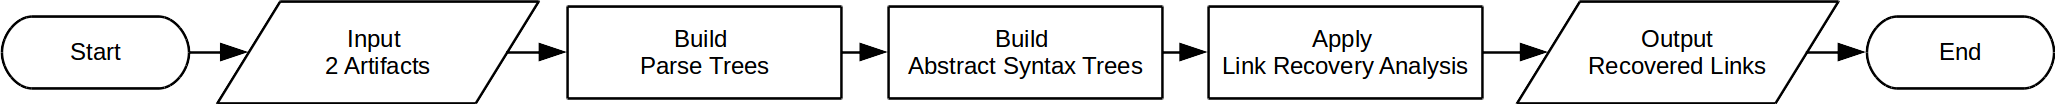
\includegraphics[width=\textwidth]{images/RecoveryProcess.png}
\end{center}
\caption{The Recovery Process}
\label{figure:RecovryProcess}
\end{figure}
Given two artifacts as input, the recovery process works as follows:
\begin{enumerate}
\item
From each artifact a \gls{CST} or \gls{ParseTree} is constructed,
\item
each \gls{ParseTree} is further refined into an \gls{AST},
\item
both \glspl{AST} are compared with each other, i.e. both trees are traversed in a \gls{DFS} fashion and each pair of nodes is checked whether it can be recovered as link.
\end{enumerate}
Eventually, the set of recovered links serves as output of the process.

\subsection{Recovery API}
The recovery \gls{API} is the core of the developed recovery system.
It provides generalized data structures and methods for syntactic analysis of artifacts and their fragments.
Figure \ref{figure:RecovryAPI} depicts the \gls{API} as block diagram.
\begin{figure}[h!]
\begin{center}
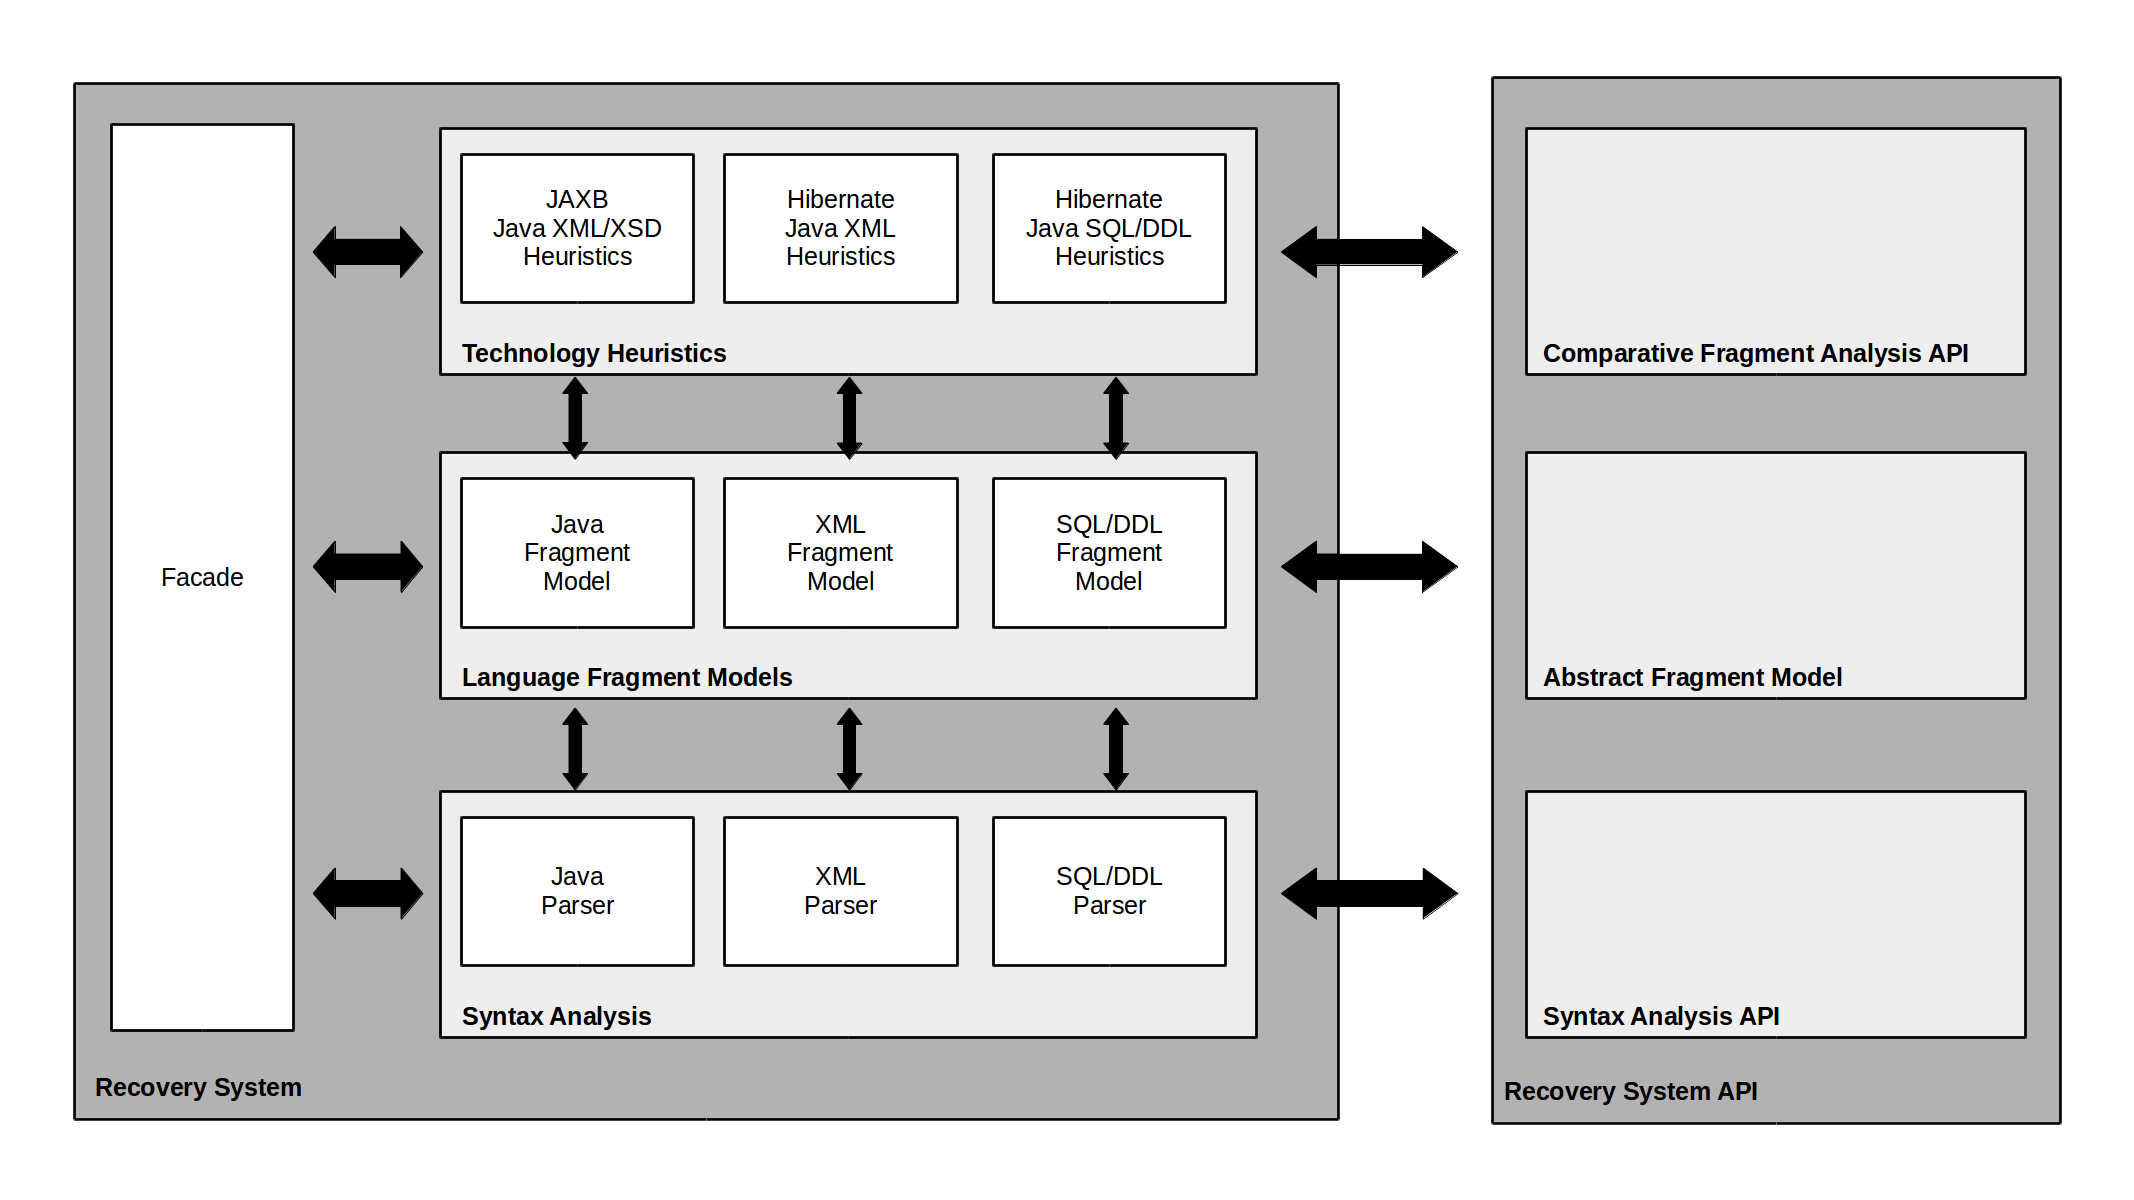
\includegraphics[width=\textwidth]{images/RecoverySystem.png}
\end{center}
{
\scriptsize
This block diagram depicts the functional outline of the Recovery System \gls{API} (note, that this does not necessarily correspond to the package outline of its actual implementation).
}
\caption{The Recovery API}
\label{figure:RecovryAPI}
\end{figure}
The components of the \gls{API} are:
\begin{description}

\item[Abstract Fragment Model]
The Abstract Fragment Model serves as base model for all \glspl{AST}.
It can thought of as \gls{DTO} for the analysis components.
As user of the \gls{API}, i have to derive a specific \gls{AST} from this model.
A detailed description follows in §\ref{subsubsection:AbstractFragmentModel}.

\item[Syntax Analysis API]
The Syntax Analysis \gls{API} is the abstraction layer for parsing and \gls{AST} construction.
It is currently backed by \gls{ANTLR}, but its internal design is loosely coupled, so other parser libraries can be used.
As user of the \gls{API}, i have to implement a parser constructing an \gls{AST} deriving the Abstract Fragment Model.
However, if one uses \gls{ANTLR}, only \gls{AST} construction from a \gls{CST} is required.
A detailed description follows in §\ref{subsubsection:SyntaxAnalysisAPI}.

\item[Fragment Analysis API]
The Fragment Analysis \gls{API} consists of two components:
\begin{description}

\item[Mereological Fragment Analysis API]
The Mereological Fragment Analysis \gls{API} provides components for deriving parthood links between syntactically well-formed fragments.
As user of the \gls{API}, i only have to apply its components to constructed \glspl{AST}.
A detailed description follows in §\ref{subsubsection:MereologicalFragmentAnalysisAPI}.

\item[Comparative Fragment Analysis API]
The Comparative Fragment Analysis \gls{API} provides components for deriving links between different artifacts and their fragments.
As user of the \gls{API}, i have to implement one or more specialized heuristics for deciding which links can be recovered.
A detailed description follows in §\ref{subsubsection:ComparativeFragmentAnalysisAPI}.

\end{description}

\end{description}

\subsubsection{Abstract Fragment Model}
\label{subsubsection:AbstractFragmentModel}
The Abstract Fragment Model describes a tree in which each node represents an syntactically well-formed fragment.
Figure \ref{figure:FragmentModel} shows an \gls{UML} class diagram of its interfaces.
\begin{figure}[h!]
\begin{center}
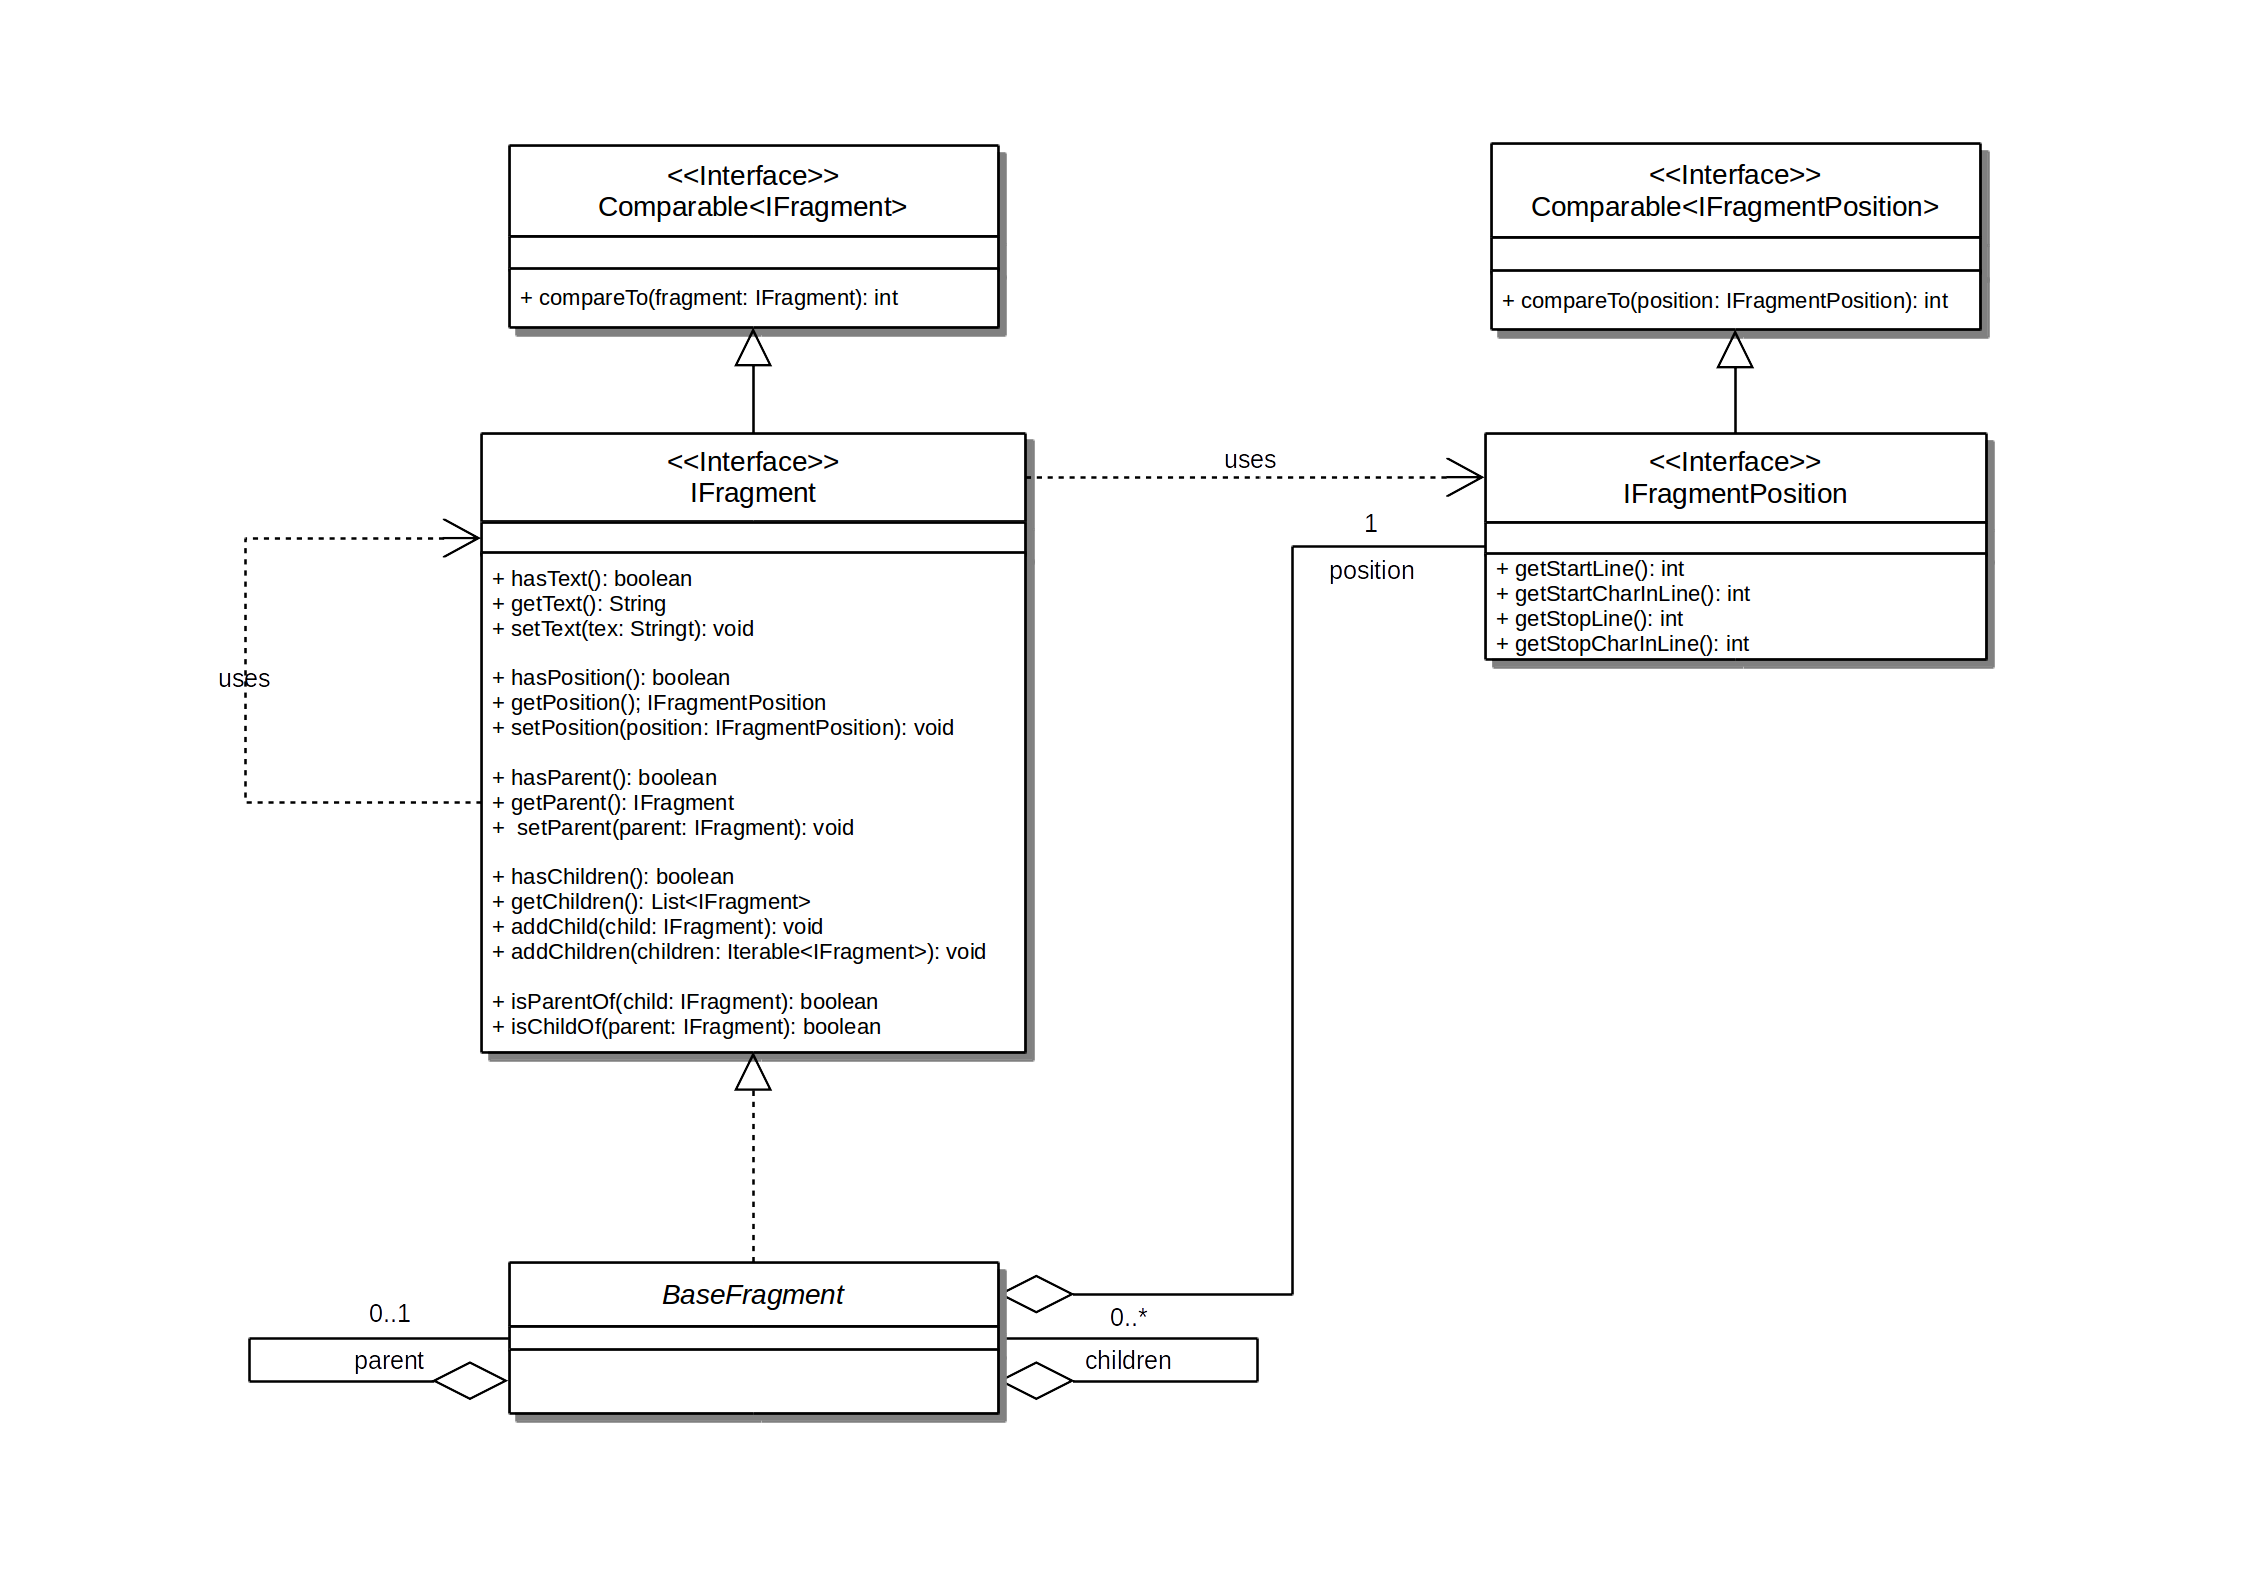
\includegraphics[width=\textwidth]{images/FragmentModel.png}
\end{center}
\caption{The Abstract Fragment Model}
\label{figure:FragmentModel}
\end{figure}
The resulting tree data structure is doubly-linked, i.e. a fragment node aggregates references to its children an to its parent, given it is not the root node.
Each fragment node contains the text it represents.
In order to distinguish fragments which represent the same text, each node also carries the text's position in the artifact.

\subsubsection{Syntax Analysis API}
\label{subsubsection:SyntaxAnalysisAPI}
The Syntax Analysis \gls{API} provides abstraction for \gls{AST} construction.
The \gls{API} itself is really small, it only consists of the \texttt{IParser} and \texttt{IParserFactory} interfaces.
However, its implementation for \gls{ANTLR} is designed to reduce \gls{ANTLR}-specific boilerplate code.
Figure \ref{figure:SyntaxAnalysisAPI} shows the \gls{UML} class diagram for the \gls{ANTLR} backed implementation.
\begin{figure}[h!]
\begin{center}
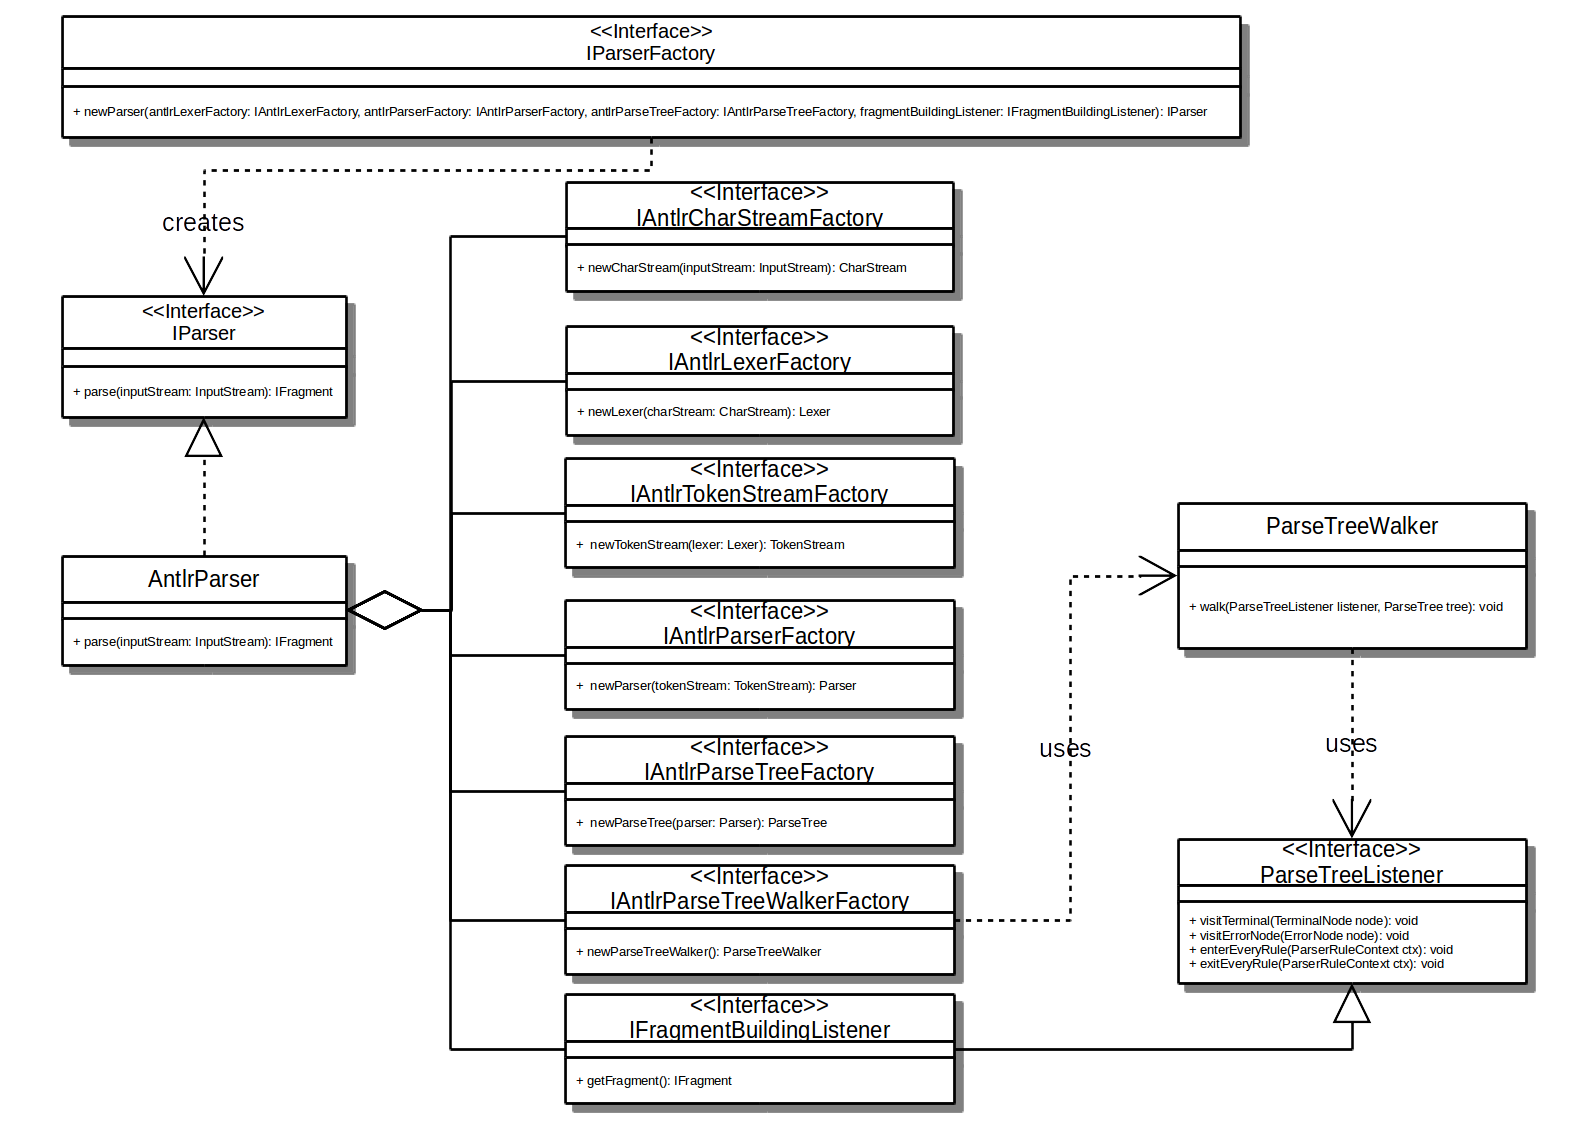
\includegraphics[width=\textwidth]{images/SyntaxAnalysisAPI.png}
\end{center}
\caption{The Syntax Analysis API}
\label{figure:SyntaxAnalysisAPI}
\end{figure}
One can see, that this implementation makes heavy use of the \gls{AbstractFactoryPattern}.
This allows for a quick and easy definition of new parsers as shown in Figure \ref{figure:IParserFactoryUsageExample}.

\begin{figure}[h!]
\begin{lstlisting}
...
IParser java8Parser = parserFactory.newParser(
	Java8Lexer::new,
	Java8Parser::new, 
	Java8Parser::compilationUnit, 
	Java8FragmentBuildingListener::new);
...
\end{lstlisting}
{
\scriptsize
This example demonstrates the creation of a new parser using an \texttt{IParserFactory} instance with \gls{Java}8 features.
Lexer and Parser classes are generated by \gls{ANTLR}.
A suitable listener has to be implemented.
}
\caption{\texttt{IParserFactory} Usage Example}
\label{figure:IParserFactoryUsageExample}
\end{figure}

The other advantage of the \gls{AbstractFactoryPattern} is that the instantiation of all relevant classes necessary for the creation of \gls{ANTLR} \glspl{ParseTree} takes place in the predefined \texttt{AntlrParser} class.
This is exemplified by Figure \ref{figure:AntlrParserParseTreeCreation}.

\begin{figure}[h!]
\begin{lstlisting}
...
CharStream charStream = antlrCharStreamFactory.newCharStream(inputStream);
Lexer lexer = antlrLexerFactory.newLexer(charStream);
TokenStream tokenStream = antlrTokenStreamFactory.newTokenStream(lexer);
Parser parser = antlrParserFactory.newParser(tokenStream);
ParseTree parseTree = antlrParseTreeFactory.newParseTree(parser);
...
\end{lstlisting}
{
\scriptsize
This example demonstrates the creation of an \gls{ANTLR} \texttt{ParseTree} instance as implemented by the \texttt{AntlrParser} class.
}
\caption{\texttt{AntlrParser} \gls{ParseTree} Creation}
\label{figure:AntlrParserParseTreeCreation}
\end{figure}

Creation of \glspl{AST} or fragment trees is done using the \texttt{ParseTreeWalker} and \texttt{ParseTreeListener} infrastructure provided by \gls{ANTLR} \cite{Parr:2013:DAR:2501720}.
This is an variation of the \gls{ObserverPattern} and alternative to the \gls{VisitorPattern}.
An instance of \texttt{ParseTreeWalker} traverses an \gls{ParseTree} using \gls{DFS}.
During traversal, a designated method of \texttt{ParseTreeListener} is executed.
For \gls{AST} creation, an \gls{API} user has to implement the \texttt{IFragmentBuildingListener} interface, which is an extension of the \texttt{ParseTreeListener} interface.
The creation of a fragment tree by \texttt{AntlrParser} is exemplified in Figure \ref{figure:AntlrParserFragmentCreation}.

\begin{figure}[h!]
\begin{lstlisting}
...
ParseTreeWalker parseTreeWalker = antlrParseTreeWalkerFactory.newParseTreeWalker();
parseTreeWalker.walk(fragmentBuildingListener, parseTree);
IFragment fragment = fragmentBuildingListener.getFragment();
...
\end{lstlisting}
{
\scriptsize
This example demonstrates the creation of an \texttt{IFragment} \gls{AST} instance as implemented by the \texttt{AntlrParser} class.
}
\caption{\texttt{AntlrParser} Fragment Creation}
\label{figure:AntlrParserFragmentCreation}
\end{figure}

\subsubsection{Mereological Fragment Analysis API}
\label{subsubsection:MereologicalFragmentAnalysisAPI}

\subsubsection{Comparative Fragment Analysis API}
\label{subsubsection:ComparativeFragmentAnalysisAPI}

\subsection{Recovery System}

\section{Megal/Xtext Integration Design}
This section summarizes the design of the recovery system's integration in the \gls{MegaL/Xtext} environment.
